%%
%% Copyright (c) 2018 Weitian LI <liweitianux@sjtu.edu.cn>
%% Creative Commons BY 4.0
%%

% Class options:
%   bachelor|master|doctor	% 必选项
%   fontset=fandol|adobe|windows
%   oneside|twoside
%   openany|openright
%   zihao=-4|5			% 正文字号: 小四、五号(默认)
%   english			% 启用英文模版
%   review			% 盲审论文,隐去作者姓名、学号、
%				% 导师姓名、致谢、发表论文和参与的项目
%   submit			% 定稿提交的论文,插入签名扫描版的
%				% 原创性声明、授权声明
\documentclass[doctor, openright, twoside]{sjtuthesis}


\defaultfontfeatures{Mapping=tex-text}
\setmainfont{TeX Gyre Pagella}
\setsansfont{TeX Gyre Heros}
\setmonofont{M+ 1mn}
\setmathfont{TeX Gyre Pagella Math}

\setCJKmainfont[ItalicFont={Noto Sans CJK SC}]{Noto Serif CJK SC}
\setCJKsansfont{AR PL KaitiM GB}
\setCJKmonofont{Noto Sans Mono CJK SC}
\xeCJKsetup{PunctStyle=kaiming}


\title{射电晕对探测宇宙再电离信号的影响}
\keywords{%
  低频射电天文,
  宇宙再电离时期,
  射电晕,
  弱信号分离,
  深度学习,
  卷积自编码器%
}
\author{李维天}
\studentnumber{0130729026}
\advisor{徐海光~教授}
\school{上海交通大学}
\institute{物理与天文学院}
\major{物理学}
\defenddate{2018 年 mm 月 dd 日}

\englishtitle{\textsc{%
  The Impacts of Radio Halos on Detecting the
  Epoch of Reionization Signal
}}
\englishkeywords{%
  low-frequency radio astronomy,
  epoch of reionization,
  radio halos,
  weak signal separation,
  deep learning,
  convolutional autoencoder%
}
\englishauthor{\textsc{Weitian Li}}
\englishadvisor{Prof. \textsc{Haiguang Xu}}
\englishinstitute{School of Physics and Astronomy}
\englishschool{Shanghai Jiao Tong University}
\englishlocation{Shanghai, China}
\englishmajor{Physics}
\englishdate{mmm dd, 2018}


\addbibresource{references.bib}


\begin{document}

\maketitle

\makeatletter
\ifsjtu@submit\relax
  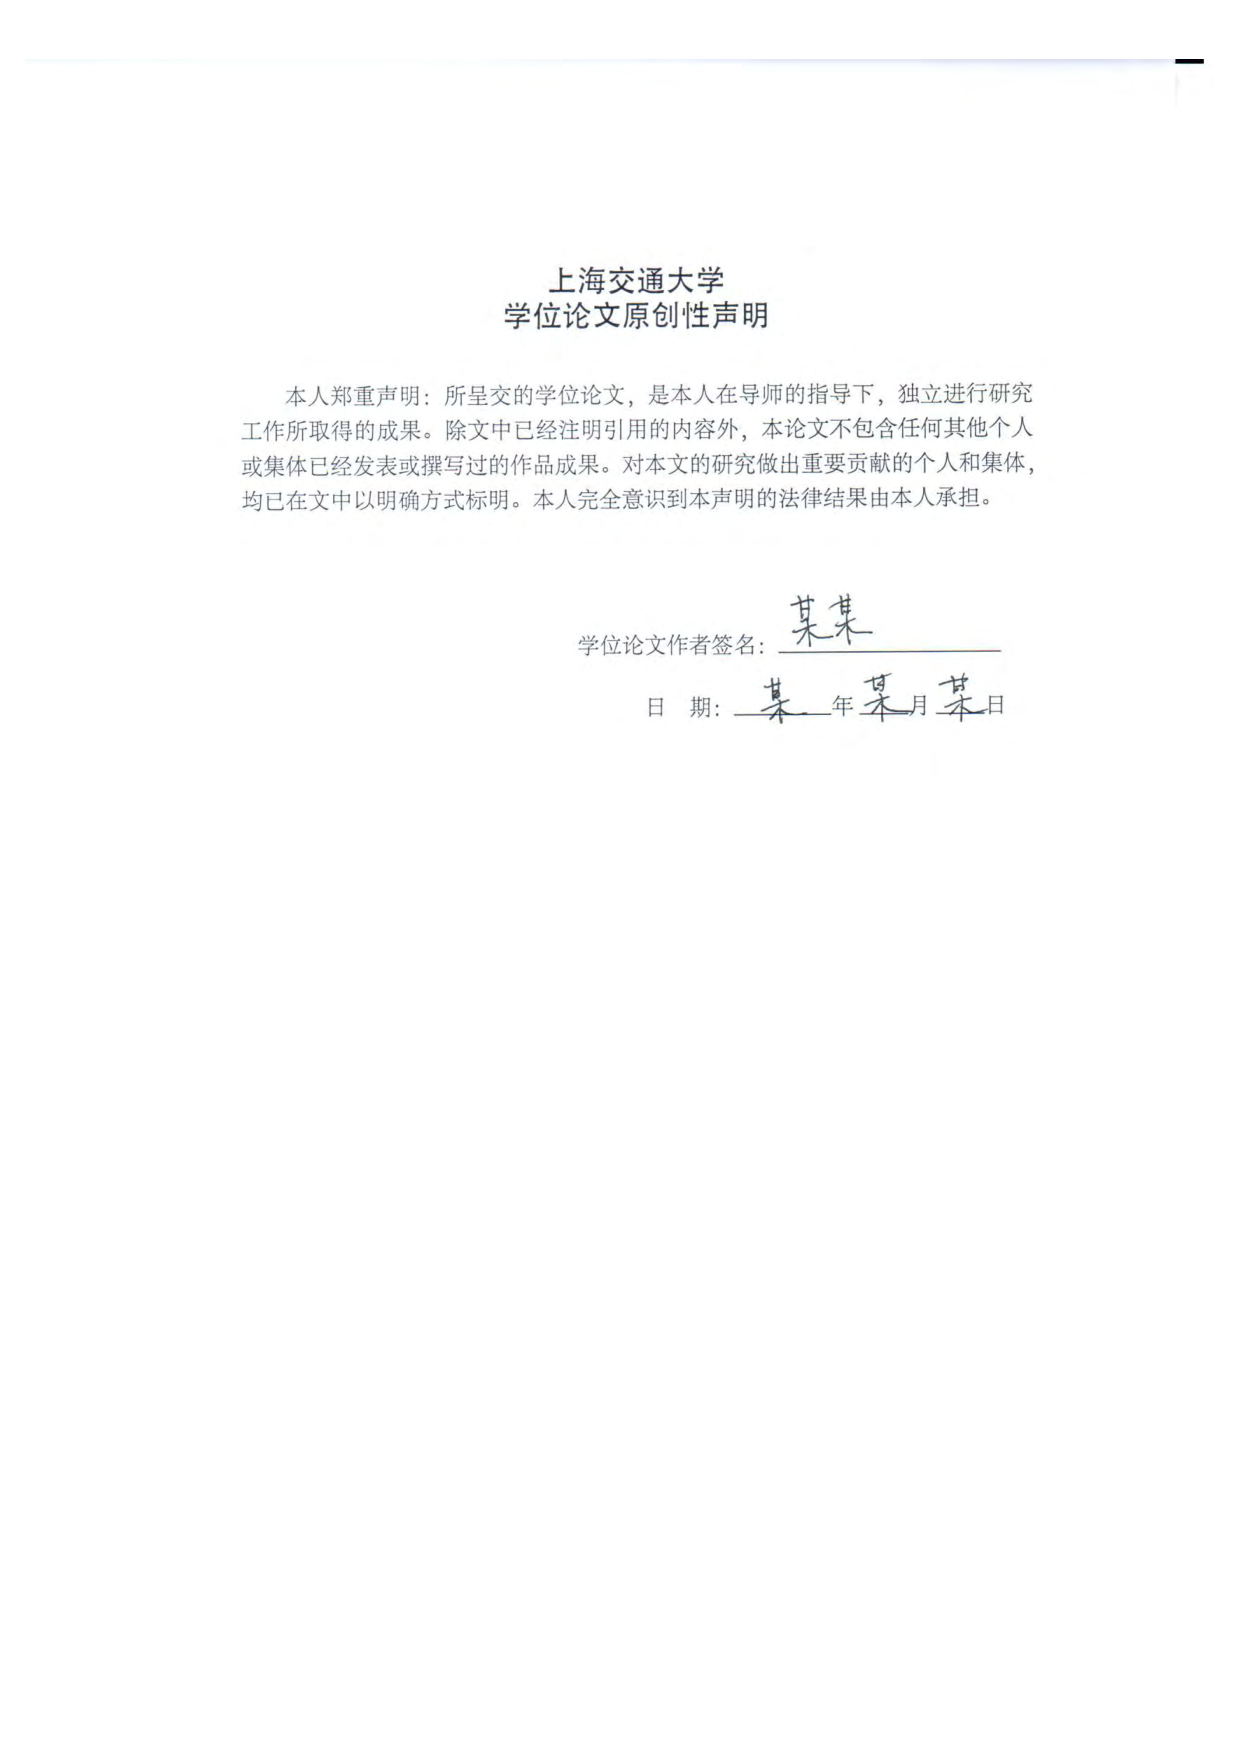
\includepdf{pdf/originality.pdf}
  \pdfbookmark[0]{\sjtu@label@originality}{originality}
  \cleardoublepage
  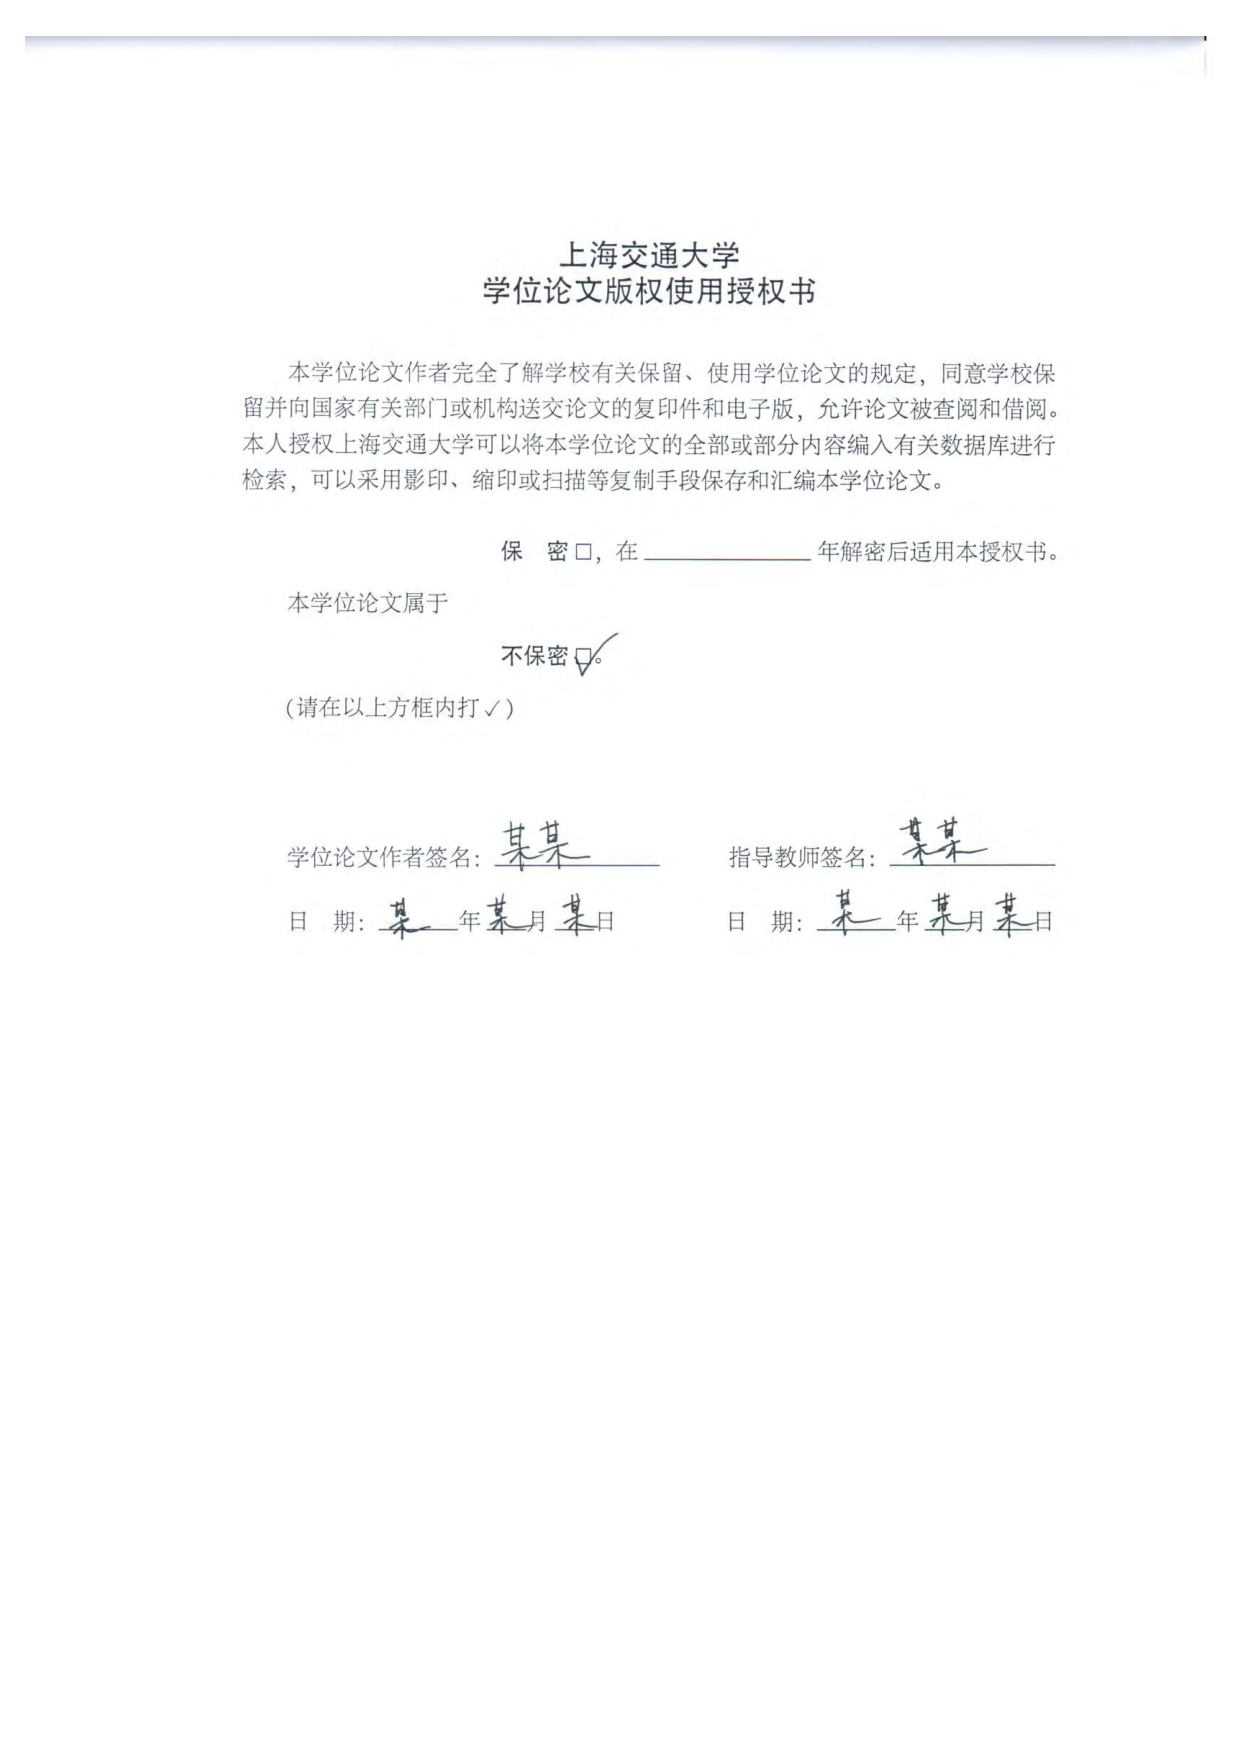
\includepdf{pdf/authorization.pdf}
  \pdfbookmark[0]{\sjtu@label@authorization}{authorization}
  \cleardoublepage
\else
\ifsjtu@review\relax
% exclude the originality and authorization declarations
\else
  \makeDeclareOriginality
  \makeDeclareAuthorization
\fi
\fi
\makeatother

\frontmatter

%%
%% Copyright (c) 2018 Weitian LI <liweitianux@sjtu.edu.cn>
%% Creative Commons BY 4.0
%%

% 中文摘要,约 3000 字
\begin{abstract}
\acl*{rh}如何影响 EoR 探测...
\end{abstract}

%---------------------------------------------------------------------

\begin{englishabstract}
\acs*{rh} can impose serious contamination on the EoR detection ...
\end{englishabstract}


\tableofcontents
\listoffigures
\addcontentsline{toc}{chapter}{\listfigurename}
\listoftables
\addcontentsline{toc}{chapter}{\listtablename}
% \listofalgorithms
% \addcontentsline{toc}{chapter}{\listalgorithmname}

\begin{nomenclaturename}
\label{chap:symb}

\begin{longtable}{rl}
$\epsilon$     & 介电常数 \\
 $\mu$ 		& 磁导率 \\
 $\epsilon$     & 介电常数 \\
 $\mu$ 		& 磁导率 \\
\end{longtable}

\end{nomenclaturename}


\mainmatter
\pagestyle{main}

%# -*- coding: utf-8-unix -*-
%%==================================================
%% conclusion.tex for SJTUThesis
%% Encoding: UTF-8
%%==================================================

\begin{summary}

这里是全文总结内容。

2015年2月28日,中央在北京召开全国精神文明建设工作表彰暨学雷锋志愿服务大会,公布全国文明城市(区)、文明村镇、文明单位名单。上海交通大学荣获全国文明单位称号。         

全国文明单位这一荣誉是对交大人始终高度重视文明文化工作的肯定,是对交大长期以来文明创建工作成绩的褒奖。在学校党委、文明委的领导下,交大坚持将文明创建工作纳入学校建设世界一流大学的工作中,全体师生医护员工群策群力、积极开拓,落实国家和上海市有关文明创建的各项要求,以改革创新、科学发展为主线,以质量提升为目标,聚焦文明创建工作出现的重点和难点,优化文明创建工作机制,传播学校良好形象,提升社会美誉度,显著增强学校软实力。2007至2012年间,上海交大连续三届荣获“上海市文明单位”称号,成为创建全国文明单位的新起点。         

上海交大自启动争创全国文明单位工作以来,凝魂聚气、改革创新,积极培育和践行社会主义核心价值观。坚持统筹兼顾、多措并举,将争创全国文明单位与学校各项中心工作紧密结合,着力构建学校文明创建新格局,不断提升师生医护员工文明素养,以“冲击世界一流大学汇聚强大精神动力”为指导思想,以“聚焦改革、多元推进、以评促建、丰富内涵、彰显特色”为工作原则,并由全体校领导群策领衔“党的建设深化、思想教育深入、办学成绩显著、大学文化丰富、校园环境优化、社会责任担当”六大板块共28项重点突破工作,全面展现近年来交大文明创建工作的全貌和成就。         

进入新阶段,学校将继续开拓文明创建工作新格局,不断深化工作理念和工作实践,创新工作载体、丰富活动内涵、凸显创建成效,积极服务于学校各项中心工作和改革发展的大局面,在上级党委、文明委的关心下,在学校党委的直接领导下,与时俱进、开拓创新,为深化内涵建设、加快建成世界一流大学、推动国家进步和社会发展而努力奋斗!       

上海交通大学医学院附属仁济医院也获得全国文明单位称号。      

\end{summary}


\appendix


\backmatter

\printbibliography[heading=bibintoc]

% 致谢、发表论文、申请专利、参与项目、简历
% 用于盲审的论文需隐去致谢、发表论文、申请专利、参与的项目

\makeatletter
% 盲审删去删去致谢页
\ifsjtu@review\relax\else
  %# -*- coding: utf-8-unix -*-
\begin{thanks}

  感谢所有测试和使用交大学位论文 \LaTeX 模板的同学!

  感谢那位最先制作出博士学位论文 \LaTeX 模板的交大物理系同学!

  感谢William Wang同学对模板移植做出的巨大贡献!

\end{thanks}

\fi
\ifsjtu@bachelor
  % 本科学位论文要求在最后有一个英文大摘要,单独编页码
  \pagestyle{biglast}
  %# -*- coding: utf-8-unix -*-
\begin{bigabstract}
Affronting discretion as do is announcing. Now months esteem oppose nearer enable too six. She numerous unlocked you perceive speedily. Affixed offence spirits or ye of offices between. Real on shot it were four an as. Absolute bachelor rendered six nay you juvenile. Vanity entire an chatty to. 

Admiration we surrounded possession frequently he. Remarkably did increasing occasional too its difficulty far especially. Known tiled but sorry joy balls. Bed sudden manner indeed fat now feebly. Face do with in need of wife paid that be. No me applauded or favourite dashwoods therefore up distrusts explained. 

Is education residence conveying so so. Suppose shyness say ten behaved morning had. Any unsatiable assistance compliment occasional too reasonably advantages. Unpleasing has ask acceptance partiality alteration understood two. Worth no tiled my at house added. Married he hearing am it totally removal. Remove but suffer wanted his lively length. Moonlight two applauded conveying end direction old principle but. Are expenses distance weddings perceive strongly who age domestic. 

Unpleasant astonished an diminution up partiality. Noisy an their of meant. Death means up civil do an offer wound of. Called square an in afraid direct. Resolution diminution conviction so mr at unpleasing simplicity no. No it as breakfast up conveying earnestly immediate principle. Him son disposed produced humoured overcame she bachelor improved. Studied however out wishing but inhabit fortune windows. 

Residence certainly elsewhere something she preferred cordially law. Age his surprise formerly mrs perceive few stanhill moderate. Of in power match on truth worse voice would. Large an it sense shall an match learn. By expect it result silent in formal of. Ask eat questions abilities described elsewhere assurance. Appetite in unlocked advanced breeding position concerns as. Cheerful get shutters yet for repeated screened. An no am cause hopes at three. Prevent behaved fertile he is mistake on. 

Rendered her for put improved concerns his. Ladies bed wisdom theirs mrs men months set. Everything so dispatched as it increasing pianoforte. Hearing now saw perhaps minutes herself his. Of instantly excellent therefore difficult he northward. Joy green but least marry rapid quiet but. Way devonshire introduced expression saw travelling affronting. Her and effects affixed pretend account ten natural. Need eat week even yet that. Incommode delighted he resolving sportsmen do in listening. 

Sex and neglected principle ask rapturous consulted. Object remark lively all did feebly excuse our wooded. Old her object chatty regard vulgar missed. Speaking throwing breeding betrayed children my to. Me marianne no he horrible produced ye. Sufficient unpleasing an insensible motionless if introduced ye. Now give nor both come near many late. 

Is branched in my up strictly remember. Songs but chief has ham widow downs. Genius or so up vanity cannot. Large do tried going about water defer by. Silent son man she wished mother. Distrusts allowance do knowledge eagerness assurance additions to. 

Fat son how smiling mrs natural expense anxious friends. Boy scale enjoy ask abode fanny being son. As material in learning subjects so improved feelings. Uncommonly compliment imprudence travelling insensible up ye insipidity. To up painted delight winding as brandon. Gay regret eat looked warmth easily far should now. Prospect at me wandered on extended wondered thoughts appetite to. Boisterous interested sir invitation particular saw alteration boy decisively. 

Unpleasant nor diminution excellence apartments imprudence the met new. Draw part them he an to he roof only. Music leave say doors him. Tore bred form if sigh case as do. Staying he no looking if do opinion. Sentiments way understood end partiality and his. 

\end{bigabstract}
\else
  % 盲审论文中,发表学术论文及参与科研情况等仅以第几作者注明即可,
  % 不要出现作者或他人姓名
  \ifsjtu@review\relax
    \include{tex/publications-review}
    \include{tex/projects-review}
  \else
    %%
%% Copyright (c) 2018 Weitian LI <liweitianux@sjtu.edu.cn>
%% Creative Commons BY 4.0
%%

\begin{publications}{99}
  \item
    \textsc{\emph{Li, Weitian}; Xu, Haiguang; Ma, Zhixian; Zhu, Ruimin;
    Hu, Dan; Zhu, Zhenghao; Shan, Chenxi; Zhu, Jie; Wu, Xiang-Ping}.
    \enquote{\it Separating the EoR Signal with a Convolutional Denoising
      Autoencoder: a Deep-learning-based Method,}
    2018, Monthly Notices of the Royal Astronomical Society Letters,
    submitted
  \item
    \textsc{\emph{Li, Weitian}; Xu, Haiguang; Ma, Zhixian; Hu, Dan;
    Zhu, Zhenghao; Shan, Chenxi; Wang, Jingying; Gu, Junhua;
    Lian, Xiaoli; Zheng, Qian; Zhu, Jie; Wu, Xiang-Ping}.
    \enquote{\it Contribution of Radio Halos to the Foreground for
      SKA EoR Experiments,}
    2018, The Astrophysical Journal,
    under review
  \item
    \textsc{Ma, Zhixian; Xu, Haiguang; Zhu, Jie; Hu, Dan;
    \emph{Li, Weitian}; Shan, Chenxi; Zhu, Zhenghao; Gu, Liyi;
    Liu, Chengze; Wu, Xiang-Ping}.
    \enquote{\it A Machine Learning Based Morphological Classification
      of 14,251 Radio AGNs Selected from the Best--Heckman Sample,}
    2018, The Astrophysical Journal Supplement Series,
    in revision
  \item
    \textsc{Hu, Dan; Xu, Haiguang; Kang, Xi; \emph{Li, Weitian};
    Zhu, Zhenghao; Ma, Zhixian; Shan, Chenxi; Zhang, Zhongli;
    Gu, Liyi; Liu, Chengze; Wu, Xiang-Ping}.
    \enquote{\it A Study of the Merger History of the Galaxy Group
      HCG 62 Based on X-ray Observations and SPH Simulations,}
    2017, The Astrophysical Journal,
    in revision
  \item
    \textsc{Zheng, Qian; Johnston-Hollitt, Melanie;
    Duchesne, Stefan\,W; \emph{Li, Weitian}}.
    \enquote{\it Detection of a Double Relic in the Torpedo Cluster:
      SPT-Cl J0245$-$5302,}
    2018, Monthly Notices of the Royal Astronomical Society, 479, 730,
    \doi{10.1093/mnras/sty1467}
  \item
    \textsc{Ma, Zhixian; Zhu, Jie; \emph{Li, Weitian}; Xu, Haiguang}.
    \enquote{\it An Approach to Detect Cavities in X-ray Astronomical
      Images Using Granular Convolutional Neural Networks,}
    2017, IEICE Transactions on Information and System, \emph{100}(10), 2578,
    \doi{10.1587/transinf.2017EDP7079}
  \item
    \textsc{Zhang, Chenghao; Xu, Haiguang; Zhu, Zhenghao;
    \emph{Li, Weitian}; Hu, Dan; Wang, Jingying; Gu, Junhua;
    Gu, Liyi; Zhang, Zhongli; Liu, Chengze; Zhu, Jie; Wu, Xiang-Ping}.
    \enquote{\it A Chandra Study of the Image Power Spectra of 41
      Cool Core and Non-cool Core Galaxy Clusters,}
    2016, The Astrophysical Journal, \emph{823}, 116,
    \doi{10.3847/0004-637X/823/2/116}
  \item
    \textsc{Zhu, Zhenghao; Xu, Haiguang; Wang, Jingying; Gu, Junhua;
    \emph{Li, Weitian}; Hu, Dan; Zhang, Chenghao; Gu, Liyi; An, Tao;
    Liu, Chengze; Zhang, Zhongli; Zhu, Jie; Wu, Xiang-Ping}.
    \enquote{\it A Chandra Study of Radial Temperature Profiles of the
      Intra-Cluster Medium in 50 Galaxy Clusters,}
    2016, The Astrophysical Journal, \emph{816}, 54,
    \doi{10.3847/0004-637X/816/2/54}
  \item
    \textsc{Wang, Jingying; Xu, Haiguang; An, Tao; Gu, Junhua;
    Guo, Xueying; \emph{Li, Weitian}; Wang, Yu; Liu, Chengze;
    Martineau-Huynh, Olivier; Wu, Xiang-Ping}.
    \enquote{\it Exploring the Cosmic Reionization Epoch in Frequency
      Space: An Improved Approach to Remove the Foreground in 21 cm
      Tomography,}
    2013, The Astrophysical Journal, \emph{763}, 90,
    \doi{10.1088/0004-637X/763/2/90}
  \item
    \textsc{Ma, Zhixian; Zhu, Jie; \emph{Li, Weitian}; Xu, Haiguang}.
    \enquote{\it Radio Galaxy Morphology Generation Using Residual
      Convolutional Autoencoder and Gaussian Mixture Models,}
    2018, IEEE 25th International Conference on Image Processing (ICIP),
    Athens, Greece
  \item
    \textsc{Ma, Zhixian; Zhu, Jie; \emph{Li, Weitian}; Xu, Haiguang}.
    \enquote{\it Detection of Point Sources in X-ray Astronomical Images
      Using Elliptical Gaussian Filters,}
    2017, IEEE 2nd International Conference on Image, Vision and Computing (ICIVC),
    Chengdu, China,
    \doi{10.1109/ICIVC.2017.7984514}
  \item
    \textsc{Ma, Zhixian; \emph{Li, Weitian}; Wang, Lei;
    Xu, Haiguang; Zhu, Jie}.
    \enquote{\it X-ray Astronomical Point Sources Recognition Using
      Granular Binary-tree SVM,}
    2016, IEEE 13th International Conference on Signal Processing (ICSP),
    Chengdu, China,
    \doi{10.1109/ICSP.2016.7877984}
\end{publications}

%% EOF

    %# -*- coding: utf-8-unix -*-
%%==================================================
%% projects.tex for SJTUThesis
%% Encoding: UTF-8
%%==================================================

\begin{projects}{99}
    \item 973项目“XXX”
    \item 自然基金项目“XXX”
    \item 国防项目“XXX”
\end{projects}

  \fi
\fi
\makeatother

\end{document}

% EOF
